\section{Appendix}

\subsection{Input-output analysis}
\label{app:input_ouput}


For a 2x2 economy, the $\pmb{A^d}$ matrix is equal to:
$$ \pmb{A^d} = 
\begin{pmatrix} 
	\frac{Z11}{P1}  & \frac{Z12}{P2} \\
	\frac{Z21}{P1} & \frac{Z22}{P2} 
\end{pmatrix}
=
\begin{pmatrix} 
a  & b \\
c & d
\end{pmatrix}
$$
so:
$$\pmb{\pmb{I} - \pmb{A^d}} = 
\begin{pmatrix} 
1 - d  & b \\
c & 1 - a
\end{pmatrix}
$$

We define $\Delta$ as $\Delta = det(\pmb{I} - \pmb{A^d})$. Then
$\pmb{Q} = (\pmb{I} - \pmb{A^d})^{-1}$ is equal to
$$\pmb{Q} = \frac{1}{\Delta}
\begin{pmatrix} 
1 - d  & b \\
c & 1 - a
\end{pmatrix}
$$

To get a better intuition of the mechanism, we introduce the value added per unit of production: $(va)_i = (VA_i/Pi)$.
Then, the value added per unit of final demand is equal to:
$$<va> \cdot Q =
\begin{pmatrix} 
va_1 & 0 \\
0 & va_2
\end{pmatrix}
\cdot Q 
= \frac{1}{\Delta}
\begin{pmatrix} 
va_1 \cdot (1-d) & va_1 \cdot b \\
va_2 \cdot c & va_2 \cdot (1-a)
\end{pmatrix}
$$

$$<va> \cdot Q 
= \frac{1}{\Delta}
\begin{pmatrix} 
(1- a-c)\cdot (1-d) & (1-a-c) \cdot b \\
(1-b-d) \cdot c & (1-b-d) \cdot (1-a)
\end{pmatrix}
$$

which simplifies by noting that the sum of the column are equal to 1 :
$$<va> \cdot Q 
= 
\begin{pmatrix} 
1-\theta_1 & \theta_2 \\
\theta_1  & 1-\theta_2
\end{pmatrix}
$$

with $\theta_1 =  \frac{(1-b-d) \cdot c}{(1-a)(1-d)-bc}$ and $\theta_2 = \frac{(1-a-c) \cdot b}{(1-a)(1-d)-bc}$. 
This formula reveals that the Leontief matrix allocates demand between the various sector to generate a value added. For example, an increase of $\delta$ in the demand adressed to sector S1 would generated a value added in sector S1 equal to $(1-\theta_1) \cdot \delta$, and a value added in sector S2 equal to $\theta_1 \cdot \delta$.

We can now estimate the number of job per unit of final demand. To that end, we define the vector $e$ of job per unit of value added by :
$(e_i) = (E_i/VA_i)$, where $E_i$ is the number of jobs in sector i and $VA_i$ the value added in sector i.
The number of job per unit of domestic demand - which we call domestic employment content $\pmb{ce}^d$ - is equal to:
$$(\pmb{ce^d})^t =
\pmb{e}^t \cdot <va> \cdot Q 
= 
\begin{pmatrix} 
e_1 (1-\theta_1) + e_2 \theta_1 ;&
e_1 \theta_2  + e_2 (1-\theta_2)
\end{pmatrix}
$$

This domestic employment content must now be linked to final demand. 
A shift of $\delta$ in final demand from S1 to S2 leads to a change in domestic demand equals to:
$$\pmb{d^d} =
\pmb{<1-\tau_m>} \cdot 
\begin{pmatrix} 
-\delta  \\
\delta
\end{pmatrix} 
=
\begin{pmatrix} 
- (1 - \tau_1) \\
1 - \tau_2
\end{pmatrix} \cdot \delta
$$

\subsubsection{Impacts of shifting investment}
An increase of one million euros in final demand addressed to S2 leads to an increase in jobs equal to:
$$(1-\tau_2) \cdot \left( (1-\theta_2) e_2+ \theta_2 e_1 \right)$$.

An decrease of one million euros in final demand addressed to S1 leads to an increase in jobs equal to:
$$(1-\tau_1) \cdot \left( (1-\theta_1) e_1+ \theta_1 e_2 \right)$$.

A shift in final demand of one million euros from S1 to S2 leads to an increase in employment if and only if:
$$(1-\tau_2) \cdot \left( (1-\theta_2) e_2+ \theta_2 e_1 \right) > (1-\tau_1) \cdot \left( (1-\theta_1) e_1+ \theta_1 e_2 \right)$$

It then useful to note that the right parenthesis in each side is the domestic employment content, a weighted average of direct employment intensity. The above equation can be re-written as:
$$(1-\tau_2) \cdot ce^d_2> (1-\tau_1) \cdot ce^d_1 $$
so a shift in final demand generates jobs if an only if the product of the employment content and the import rate is higher.
But the computation of the employment content shows that the domestic employment content is high if demand generates value added in sector with a high number of jobs per value added.

%%%%%%%%%%%%%%%%%%%%%%%%%%%%%%%%%%%%%%%%%%%%%%%%%%%%%%%%%%%%%%%%%%%%%%%%%%%%%%%%%%%%%%
\clearpage

\subsection{Closed economy}
\label{app:closed_economy}

\subsubsection{Overview of the closed model}
\begin{figure}[!h]
	\centering
	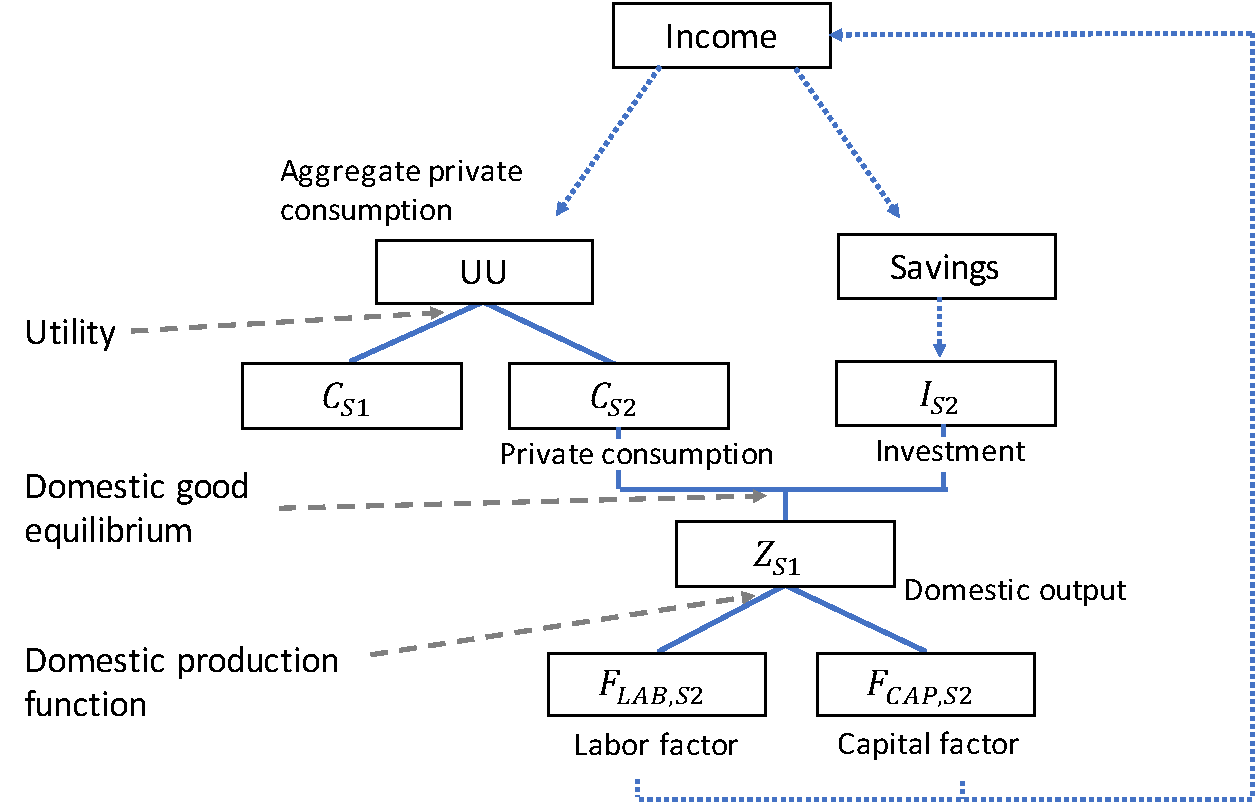
\includegraphics[height=7cm]{figures/overview_closed.pdf}
	\caption{Overview of the closed economy model for the S2 sector}
	\label{fig:overview_closed}
\end{figure}

\subsubsection{Index of sets}
\begin{itemize}
	\item $u$: S1, S2, CAP, LAB, HOH, INV
	\item $i(u)$: S1, S2. Alias: $j(u)$.
	\item $h(u)$: CAP, LAB.
\end{itemize}

\subsubsection{Index of variables}
\begin{itemize}
	
	\item $Z_j$: output of the j-th good
	\item $F_{h,j}$: the h-th factor input by the j-th firm
	\item $FF_h$: the h-th factor supply
	\item $Inc$: Household income
	\item $C_i$: household consumption of the i-th good
	\item $p^x_i$: demand price of the i-th good
	\item $p^z_i$ supply price of the i-th good
	\item $p^f_h$ the h-th factor price
	\item $pc$ consumption price index
	\item $S^p$: private savings	
	\item $U$: unemployment rate
	\item $UU$: utility (Cobb-Douglas)
\end{itemize}

\subsubsection{Index of parameters}
\begin{itemize}
	\item $\alpha_i$: share parameter in utility function
	\item $\sigma^z$: elasticity in CES production function
	\item $\rho^z = \frac{\sigma^z - 1}{\sigma^z}$: param. in CES production function
	\item $\delta_{h,j}$ share parameter in CES production function
	\item $scZ_j$: scale parameter in CES production function  
	\item $\beta_{h,j}$: share parameter in Cobb-Douglas production function
	\item $b_j$: scale parameter in Cobb-Douglas production function
	\item $a_{h,j}$: Leontief coefficient in production function
	\item $\gamma$: wage curve elasticity
	\item $U^0$: initial unemployment rate
\end{itemize}



\subsubsection{Tests}

\paragraph{Walras' law}
Walras' law allows to take off one equation. 
In our numerical application, we remove the market clearing of good for the first sector.
Then, we check after the run that Walras' law is satisfied.

\paragraph{Numéraire}
In our numerical application, we use the price index of consumption goods as the numéraire. 
We check that the model is not sensitive to this assumption. We increase the numéraire by 10\% and rerun the model.
With this assumption, we check that all prices have increased by 10\%, and volumes remain the same.

%%%%%%%%%%%%%%%%%%%%%%%%%%%%%%%%%%%%%%%%%%%%%%%%%%%%%%%%%%%%%%%%%%%%%%%%%%%%%%%%%%%%%%

\clearpage

\subsection{Simple CGE with two labor skills}
\label{app:two_labour_model}

\subsubsection{Overview of the simple CGE with two labor skills}
\begin{figure}[!h]
	\centering
	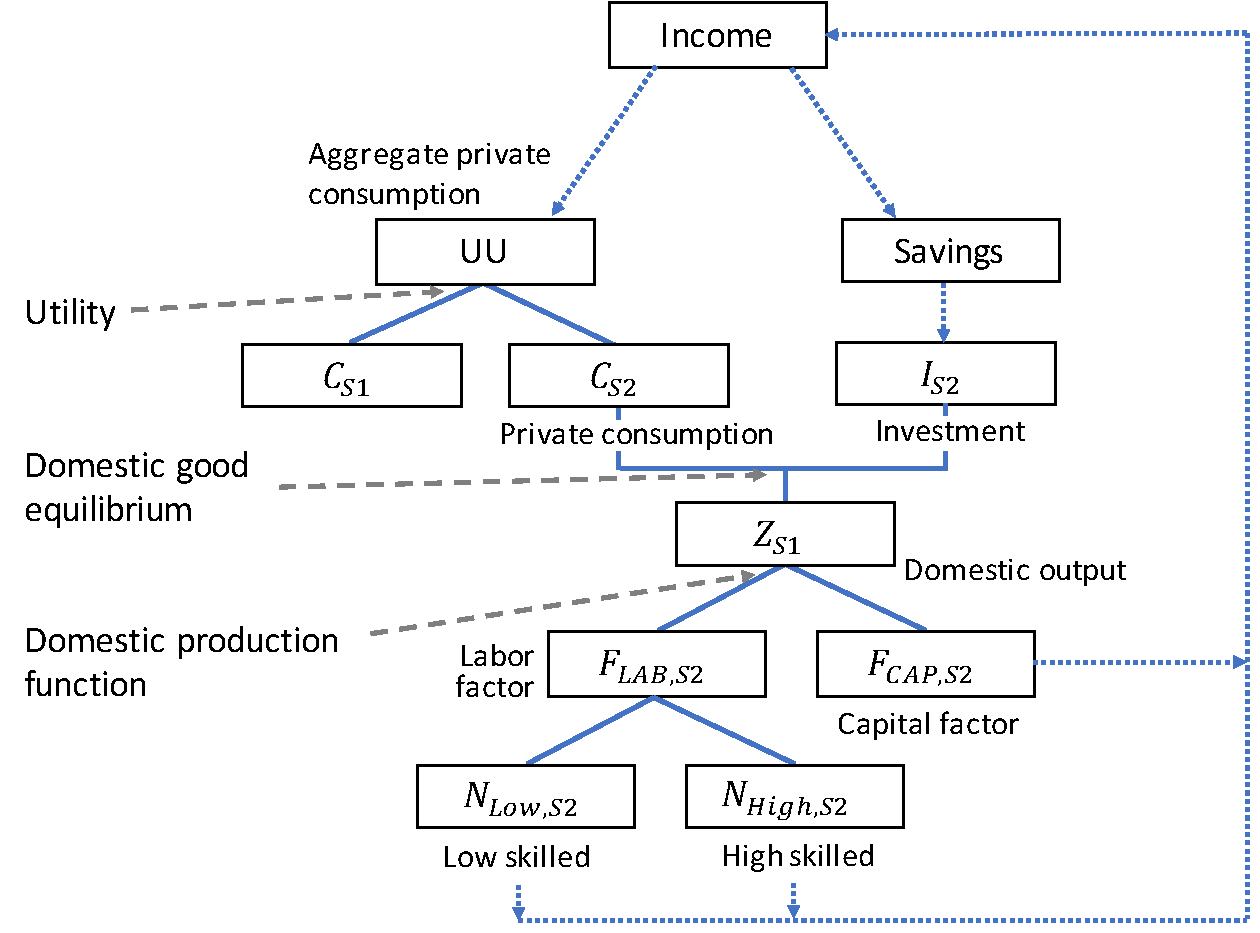
\includegraphics[height=8cm]{figures/overview_twoLabors.pdf}
	\caption{Overview of the open economy model for the S2 sector}
	\label{fig:overview_twoLabors}
\end{figure}

\subsubsection{Index of sets}
\begin{itemize}
	\item $u$: S1, S2, CAP, LAB, HOH, INV
	\item $i(u)$: S1, S2. Alias: $j(u)$
	\item $h(u)$: CAP, LAB
	\item $s$: LABL, LABH 
\end{itemize}


%%%%%%%%%%%%%%%%%%%%%%%%%%%%%%%%%%%%%%%%%%%%%%%%%%%%%%%%%%%%%%%%%%%%%%%%%%%%%%%%%%%%%%



\clearpage

\subsection{Open economy}
\label{app:open_economy_model}

\subsubsection{Overview of the open economy}
\begin{figure}[!h]
	\centering
	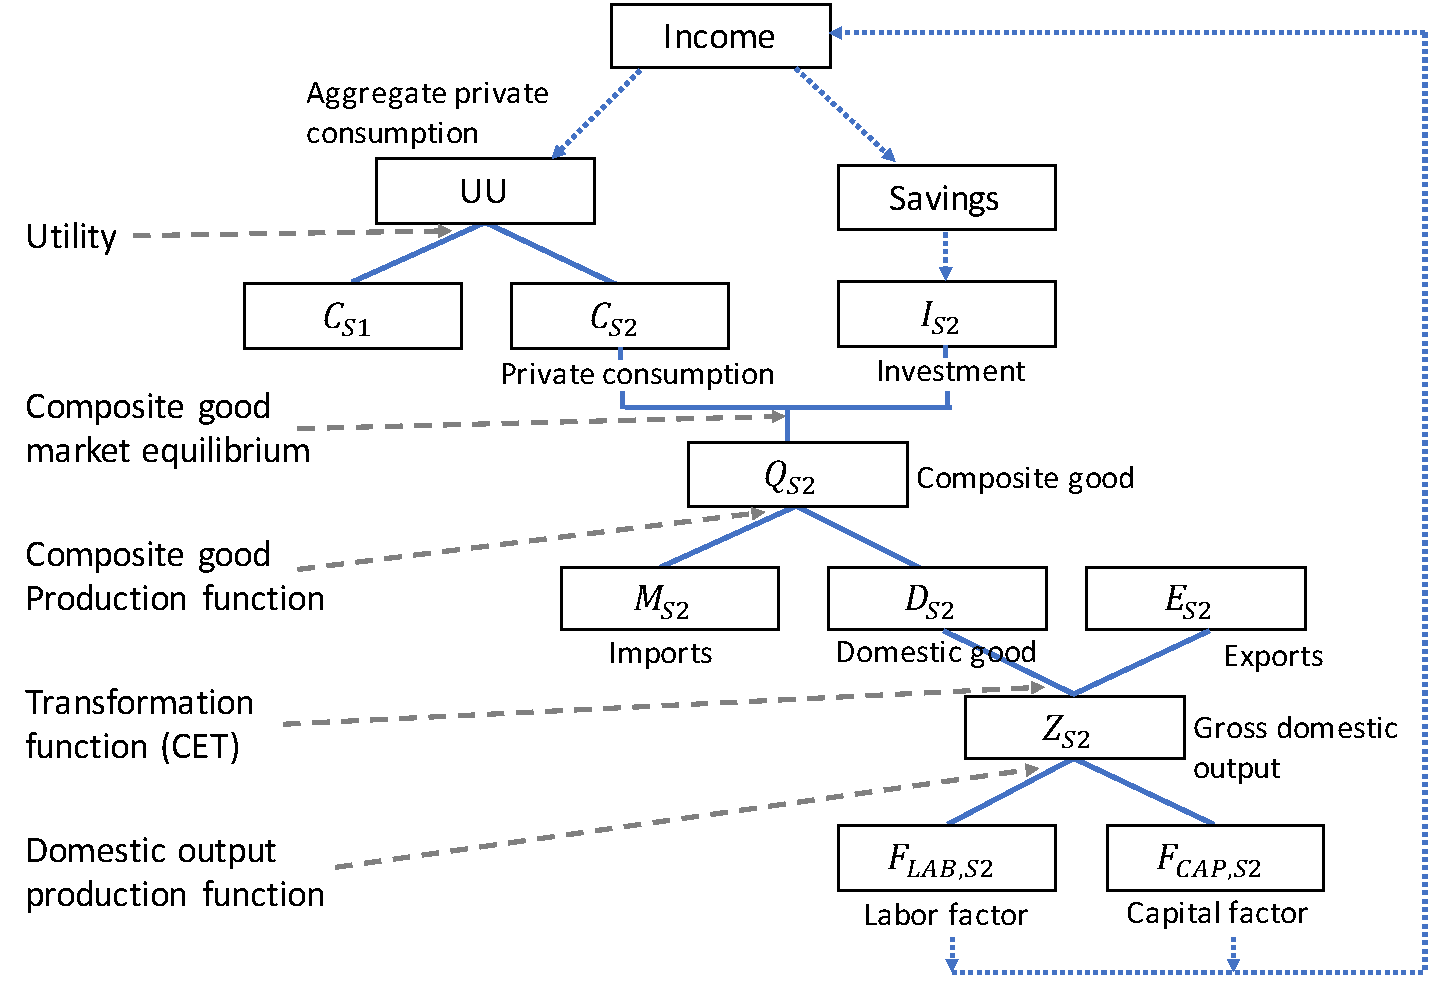
\includegraphics[height=8cm]{figures/overview_open.pdf}
	\caption{Overview of the open economy model for the S2 sector}
	\label{fig:overview_open}
\end{figure}

\subsubsection{Index of sets}
\begin{itemize}
	\item $u$: S1, S2, CAP, LAB, HOH, INV, EXT
	\item $i(u)$: S1, S2
	\item $h(u)$: CAP, LAB
\end{itemize}

\subsubsection{Index of variables}
\begin{itemize}
	\item $Z_j$: output of the j-th good
	\item $FF_h$: factor supply
	\item $F_{h,j}$: the h-th factor input by the j-th firm
	\item $Inc$: Household income
	\item $C_i$: household consumption of the i-th good
	\item $E_i$:  exports
	\item $M_i$:  imports
	\item $Q_i$:  Armingtons composite good
	\item $D_i$:  domestic good

	\item $pf_h$: the h-th factor price
	\item $p^x_i$: consumption price
	\item $p^z_j$: supply price of the i-th good
	\item $p^q_i$: Armingtons composite good price
	\item $p^e_i$: export price in local currency
	\item $p^m_i$: import price in local currency
	\item $p^d_i$: the i-th domestic good price
	\item $\epsilon$: exchange rate
	\item $p^c$: price index

	\item $S^p$: private savings
	\item $S^f$: foreign savings
	\item $U$: unemployment rate
	\item $UU$: utility (Cobb-Douglas)
\end{itemize}

\subsubsection{Index of parameters}
\begin{itemize}
	\item $\alpha^u_i$: share parameter in utility func.
	\item $\sigma^z$: elasticity in CES production function
	\item $\rho^z = \frac{\sigma^z - 1}{\sigma^z}$: param. in CES production function
	\item $\delta_{h,j}$ share parameter in CES production function
	\item $scZ_j$: scale parameter in CES production function  
	\item $\sigma^q$: elasticity of Armington substitution
	\item $\rho^q = \frac{\sigma^q-1}{\sigma^q}$: substitution elasticity parameter for Armington
	\item $\alpha^m_i$: share par. in Armington func.
	\item $\alpha^d_i$: share par. in Armington func.
	\item $scq_i$: scale par. in Armington func.
	\item $\gamma$: wage curve elasticity
	\item $U^0$: initial unemployment rate
\end{itemize}


\subsubsection{Results for IO anc CGE}
\label{subsec:open_economy_results}

\begin{table}[!h]
	\centering
	\caption{SAM results in an open economy with our IO model}
	\label{tab:SAM_IO_openEconomy}
	\begin{tabular}{llllllll}
		\toprule
		& S1 & S2 &  HOH & INV & EXT \\
		\midrule
		S1 &  &   & 8 & 5 & 3 \\
		S2 &  &    & 12 & 3 & 3 \\
		LAB & 9.60 & 8.53 &   &  &  \\
		CAP & 5.33 & 4.74 &   &  &  \\
		EXT & 1.06 & 4.74 &   &  &  \\
		\bottomrule
	\end{tabular}
\end{table}


\begin{table}[!h]
	\centering
	\caption{Open economy with fixed exchange rate $\epsilon$ and endogenous imports}
	\label{tab:SAM_IO_OpenEconomy_noBudget}
	\begin{tabular}{llllll}
		\toprule
		& S1 & S2 & HOH & INV & EXT \\
		\midrule
		S1 &  &  & 10.96 & 5.00 & 0.00 \\
		S2 &  &  & 16.44 & 3.00 & 0.00 \\
		LAB & 9.41 & 8.59 &  &  &  \\
		CAP & 5.23 & 4.77 &  &  &  \\
		EXT & 1.33 & 6.08 &  &  &  \\
		\bottomrule
	\end{tabular}
\end{table}


%%%%%%%%%%%%%%%%%%%%%%%%%%%%%%%%%%%%%%%%%%%%%%%%%%%%%%%%

\clearpage

\subsection{Full model}
\label{sec:full_model}

\subsubsection{Data}
\label{app:full_model_data}

At the 64-sector level of disaggregation, we encounter some issues to calibrate the CGE model:
\begin{itemize}
	\item Postal services (CPA\_H53) have negative capital revenues in 2013. Standard production functions with constant elasticity of substitution cannot account for a negative capital revenue. 
	Since this sector is not crucial for our analysis of green jobs, we aggregate it with the other transportation service (CPA\_H50, CPA\_H51 and CPA\_H52).
	\item The "Manufacture of textiles, wearing apparel and leather products" sector (CPA\_C13-15) and "Computer, electronic and optical products" sector (CPA\_C26) export more than they produce. To avoid issues with negative values in the calibration of trade within the constant elasticity of transformation (CET) function, we aggregate the textile and leather products with "Manufacture of wood and of products of wood" (CPA\_C16) and computers with electrical equipment (CPA\_C27)
	\item The "imputed rent" sector (CPA\_L68A) indicates a low but positive remuneration for employees, but no employee. This would lead to an infinite salary. We aggregate this sector with the other real estate services (CPA\_L68B)
\end{itemize}



\subsubsection{Overview of the full CGE model}

\begin{figure}[!h]
	\centering
	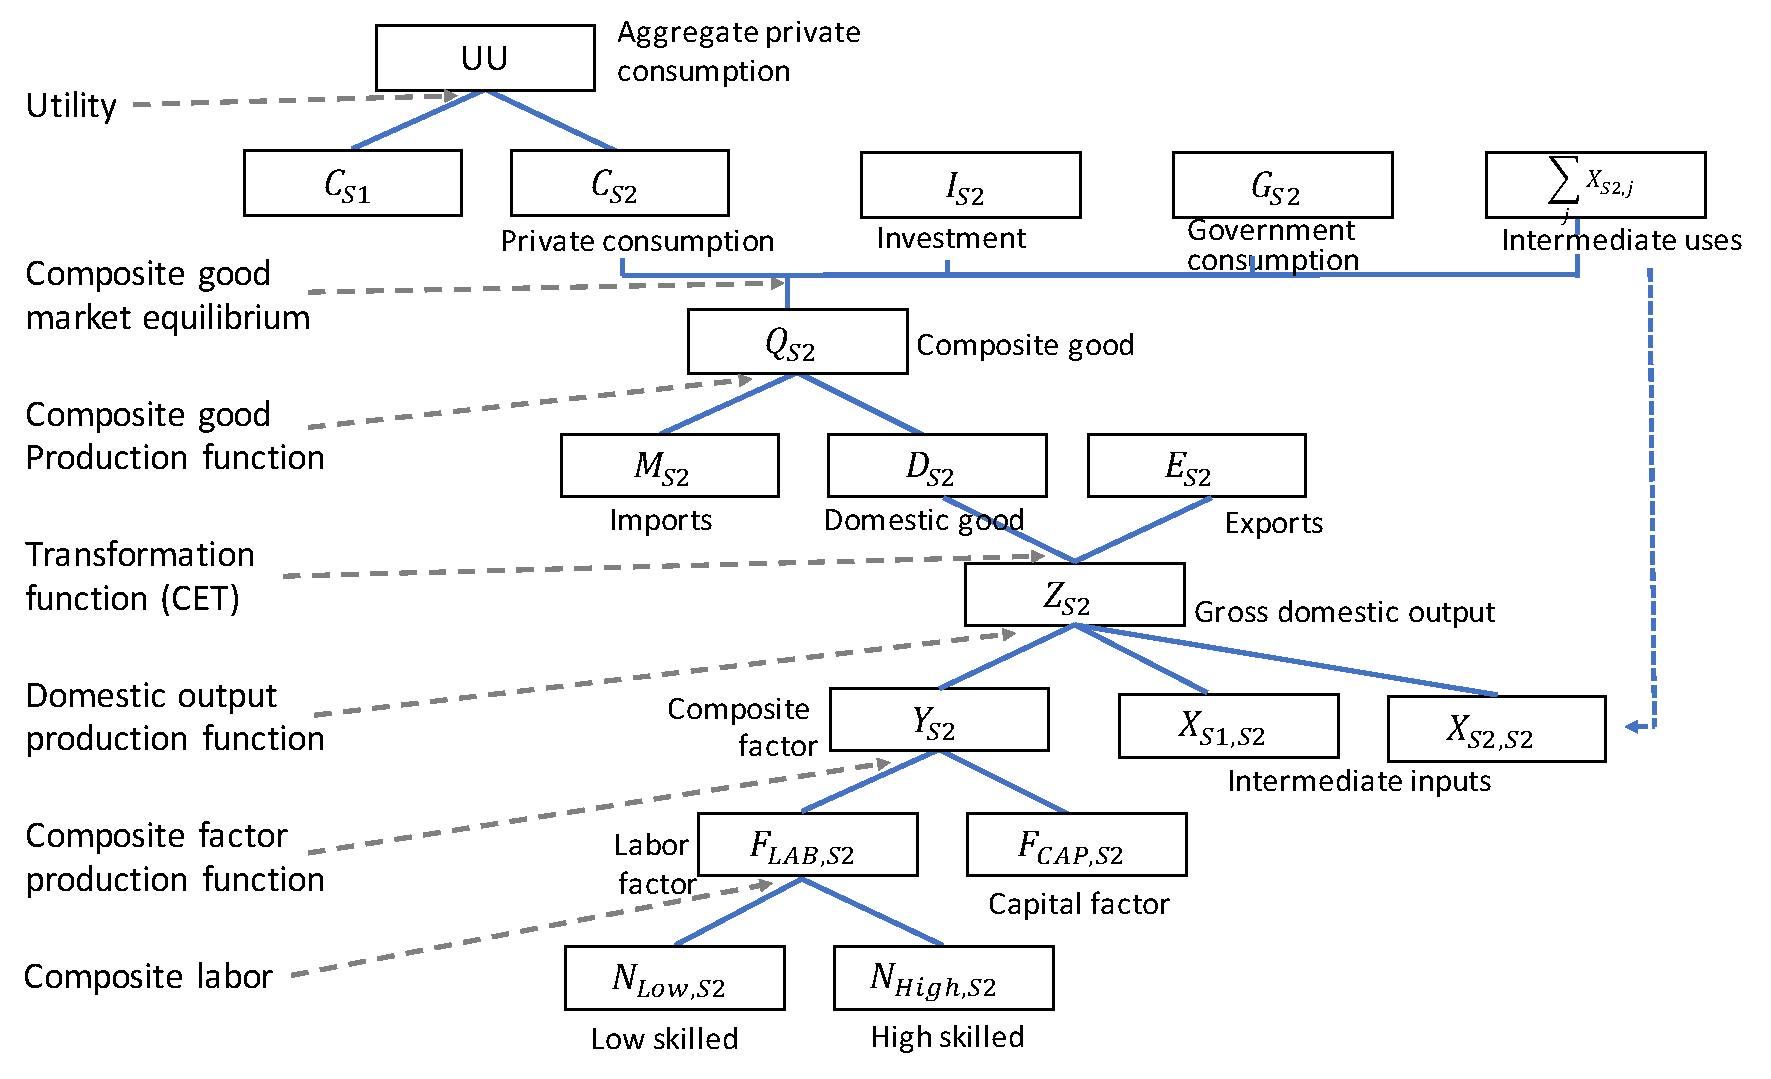
\includegraphics[width=14cm]{figures/overview_full.pdf}
	\caption{Overview of the fully-fledged model for the S2 sector}
	\label{fig:overview_full}
\end{figure}

\subsubsection{Index of sets}
\begin{itemize}
	\item u: SAM entry     /S1*S58, CAP, LAB, IDT, TRF, HOH, GOV,
	\item i(u): goods         /S1*S58/
	\item h(u): factor        /CAP, LAB/
	\item s: labor skill   / highSkill, lowSkill /
\end{itemize}

\subsubsection{Index of variables}
\begin{itemize} 
	\item $Y_j$: composite factor
	\item $Inc$: household income
	\item $N(s,j)$: worker input by skill
	\item $K_j$: capital factor input by the j-th firm
	\item $L_j$: labor input      
	\item $KK$: capital supply
	\item $NN(s)$: worker supply
	\item $X(i,j)$: intermediate input
	\item $Z_j$: output of the j-th good
	\item $C_i$: household consumption of the i-th good
	\item $G_i$: government consumption
	\item $I_i$: investment
	\item $E_i$: exports
	\item $M_i$: imports
	\item $Q_i$: Armington composite good
	\item $D_i$: domestic good

	\item $p^k$: capital factor price
	\item $p^l_j$: labor price
	\item $p^n_s$: workers price
	\item $p^y_j$: composite factor price
	\item $p^z_j$: supply price of the i-th good
	\item $p^q_i$: Armingtons composite good price
	\item $p^e_i$: export price in local currency
	\item $p^m_i$: import price in local currency
	\item $p^d_i$: the i-th domestic good price
	\item $\epsilon$: exchange rate

	\item $S^p$: private saving
	\item $S^g$: government saving
	\item $S^f$: foreign saving
	\item $T^d$: direct tax
	\item $T^z_j$: production tax
	\item $T^p$: private consumption tax
	\item $T^v$: investment tax

	\item $KK$: capital supply
	\item $NN_s$: labor supply
	\item $pc$: consumption price

	\item $UU$: utility (Cobb-Douglas)
\end{itemize}

\subsubsection{Index of parameters}
\begin{itemize}
	\item $\sigma^Y$: elasticity of substitution in composite factor production
	\item $\rho^Y = \frac{\sigma^Y - 1}{\sigma^Y}$: substitution elasticity parameter for capital-labor composite
	\item $\sigma_i$: elasticity of Armington substitution
	\item $\eta_i = \frac{\sigma^z - 1}{\sigma^z}$: substitution elasticity parameter for Armington
	\item $\psi_i$: elasticity of transformation
	\item $\phi_i= \frac{\psi^z - 1}{\psi^z}$: transformation elasticity parameter
	\item $\alpha_i$: share parameter in utility func.
	\item $\delta^l_j$: labor share   in CES prod. func.
	\item $\delta^k_j$: capital share in CES prod. func.
	\item $scY$: scale param.  in CES prod. func.
	\item $\beta\_N(s,j)$: share parameter in labor function
	\item $scL_j$: scale parameter in labor function
	\item $ax(i,j)$: intermediate input requirement coeff.
	\item $ay_j$:  composite fact. input req. coeff.
	\item $\mu_i$:  government consumption share
	\item $\lambda_i$: investment demand share
	\item $\delta^m_i$: share par. in Armington func.
	\item $\delta^d_i$: share par. in Armington func.
	\item $scQ_i$: scale par. in Armington func.
	\item $\xi^d_i$: share par. in transformation func.
	\item $\xi^e_i$: share par. in transformation func.
	\item $\theta_i$: scale par. in transformation func.
	\item $ssg$: average propensity for gov. saving
	\item $\tau^d$: direct tax rate
	\item $Pop$: population (labor force)
	\item $U^0_s$: initial unemployment
	\item $p^{We}_i$: export price in US dollars
	\item $p^{Wm}_i$: import price in US dollars
	\item $\tau^z_i$: production tax rate
	\item $\tau^p$: private consumption tax rate
	\item $\tau^v$: investment tax
	\item $Pop$: population (labor force)
	\item $\gamma$: wage curve elasticity
\end{itemize}



\begin{table}[!h]
	\centering
	\caption{Comparative equations of IO and CGE models. Identical equations are not repeated to facilitate reading. The main differences with the closed version shown in table \ref{tab:closedModel} have their equations labeled in bold.}
	\label{tab:fullModel}
	\begin{tabular}{llll}
		\toprule
		Num & Description & Standard CGE  \\
		\midrule
		eq1 & Production function & $Y_j    = scY_j \cdot  ( \delta^k_j \cdot K_j^{\rho_Y} + \delta^l_j \cdot L_j^{\rho_Y} )^(1/\rho_Y)$ \\
		eq2 & Capital demand & $ K_j = (scY_j^{\rho_Y} \cdot  \delta^k_j \cdot  p^y_j / p^k )^{\sigma_Y} \cdot  Y_j $ \\
		eq3 & Labor demand  & $L_j = (scY_j^{\rho_Y} \cdot \delta^l_j \cdot  p^y_j / p^l_j )^{\sigma_Y} \cdot Y_j $ \\	
		eq4 & Demand of intermediate goods & $X_{i,j}  = ax_{i,j} \cdot Z_j$ \\
		eq5 & Demand of composite factor & $Y_j    = ay_j \cdot Z_j$ \\
		eq6 & Condition of zero profit & $p^z_j   = ay_j \cdot p^y_j + \sum_i ax_{i,j} \cdot p^q_i$ \\
		eq7 & Production of labor composite & $L_j    = scL_j \cdot  \prod_s N_{s,j}^{\beta^N_{s,j}}$  \\
		eq8 & Demand of labor by skill & $N_{s,j}  = \beta^N_{s,j} \cdot p^l_j \cdot  L_j / p^n_s$ \\
		eq9 & Unemployment & $ U_s =  1 - NN_s/Pop_s $\\
		eq10 & Labor supply & $\log( p^n_s / p^c ) = - \gamma \cdot  log(\frac{U_s}{U^0_s}) $  \\
		eq11 & Capital supply & $KK = \overline{KK} $  \\
		\midrule
		eq12 & Direct tax on household & $T^d = \tau^d \cdot Inc $\\
		eq13 & Tax on production & $T^z_j = \tau^z_j \cdot p^z_j \cdot Z_j$ \\
		eq14 & Tax on household consumption & $T^p = \tau^p \cdot \sum_j  p^q_j \cdot C_j $ \\
		eq15 & Tax on investment & $T^v = \tau^v \cdot \sum_j p^q_j\cdot I_j $ \\
		eq16 & Government consumption & $G_i = \mu_i ~ ( T^d + \sum_j T^z_j + T^p + T^v - S^g ) / p^q_i$ \\
		\midrule
		eq17 & Private savings & $S^p = \sum_i (1+\tau^v) \cdot p^q_i \cdot I_i - S^g - \epsilon \cdot S^f$ \\
		eq18 & Government savings & $S^g = ssg \cdot  (T^d + \sum_j T^z_j + T^p + T^v)$ \\
		\midrule
		eq19 & Household income &  $Inc = p^k \cdot KK + \sum_s p^n_s \cdot NN_s $ \\
		eq20 & Houshold consumption & $C_i = \alpha_i \cdot  (Inc -S^p - T^d) / ((1+\tau^p) ~ p^q_i) $ \\
		\midrule
		eq21 & Export demand & $p^e_i = \epsilon \cdot pWe_i$ \\
		eq22 & Import supply & $p^m_i =\epsilon \cdot p^{Wm}_i$ \\
		eq23 & Balance of trade & $\sum_i p^{We}_i \cdot E_i +S^f = \sum_i p^{Wm}_i \cdot M_i$ \\
		eq24 & Trade closure & $S^f = \overline{S^f}$  \quad OR \quad $\epsilon = \overline{\epsilon}$  \\
		\midrule
		eq25 & Armington function & $Q_i = scQ_i \cdot (\alpha^m_i M_i^{\rho_Q} + \alpha^d_i D_i^{\rho_Q}  )^{1/\rho_Q} $ \\
		eq26 & Imports demand & $M_i = \left( scQ_i^{\rho_Q} \cdot \alpha_i^m \cdot \frac{p_i^q}{p_i^m} \right)^{\sigma_Q} Q_i$ \\
		eq27& Domestic demand & $D_i = \left( scQ_i^{\rho_Q} \cdot \alpha_i^d \cdot \frac{p_i^q}{p_i^d} \right)^{\sigma_Q} Q_i$ \\
		eq28 & CET function & $Z_i  = \theta_i \cdot  (\xi^e_i \cdot E_i^{\phi_i} + \xi^d_i \cdot D_i^{\phi_i} )^{(1/\phi_i)} $  \\
		eq29 & Demand of E & $  E_i = (\theta_i^{\phi_i} \cdot \xi^e_i\cdot (1+\tau^z_i) ~ p^z_i/p^e_i)^{(1/(1-\phi_i))} ~Z_i $ \\
		eq30 & Demand of D & $ D_i = (\theta_i^{\phi_i} \cdot \xi^d_i \cdot (1+\tau^z_i) ~ p^z_i/p^d_i)^{(1/(1-\phi_i))} ~ Z_i $ \\
		\midrule
		eq31 &  Balance of domestic good & $Q_i = C_i + I_i$ &  \\
		eq32 & Balance of labor & $NN_s = \sum_j N_{s,j}$ &   \\
		eq33 & Balance of capital & $KK  = \sum_j K_j $ &   \\
		eq34 & Price equality & $p^c_i = p^z_i$ & \\ 
		\bottomrule
	\end{tabular}
\end{table}

\clearpage

\subsubsection{Results}

\subsubsection{Cobb-Douglas elasticity vs Empirical estimates}

\begin{table}[!h]
	\centering
	\caption{Comparing job creation using CES vs Cobb-Douglas \\\hspace{\textwidth} (for a wage curve elasticity $\gamma$=0.1, $\sigma_{Armington}$ =2  and $\psi_{CET}$=2)}
	\label{tab:CobbDouglasError}
	\begin{tabular}{lcccc}
		\toprule
		Techno & Elasticité  &  Value & Value & Error (\%) \\
	    & $\sigma_{KL}$ &  with CES & with Cobb-Douglas& Cobb-Douglas vs CES \\
		\midrule 
		Solar & 0.2 &  5858 & 3542 & -40 \\
Solar & 0.3 &5394 & 3542 & -34 \\
Solar & 0.4 & 5003 & 3542 & -29 \\
Solar & 0.5 & 4670 & 3542 & -24 \\
Solar & 0.6 & 4382 & 3542 & -19 \\
Weatherization & 0.2 & 6589 & 4135 & -37 \\
Weatherization & 0.3 & 6097 & 4135 & -32 \\
Weatherization & 0.4 & 5683 & 4135 & -27 \\
Weatherization & 0.5 & 5331 & 4135 & -22 \\
Weatherization & 0.6 & 5026 & 4135 & -18 \\
		\bottomrule
	\end{tabular}
\end{table}

\clearpage

\subsubsection{Trade}

\begin{figure}[!h]
	\centering
	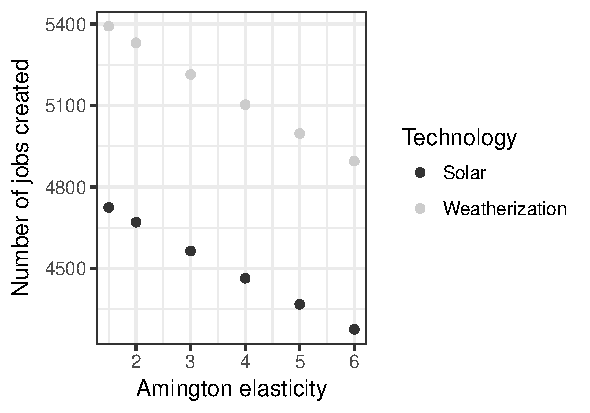
\includegraphics[height=4cm]{figures/Armington.pdf}
	\caption{Impact of the Armington elasticity (with CET elasticity equal to two)}
	\label{fig:armington}
\end{figure}

\begin{figure}[!h]
	\centering
	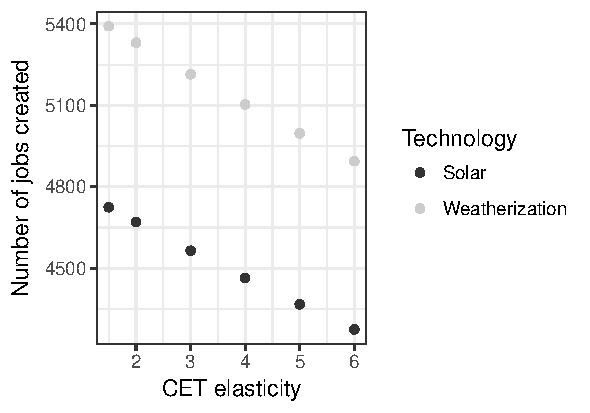
\includegraphics[height=4cm]{figures/CET.pdf}
	\caption{Impact of the CET elasticity (with Armington elasticity equal to two)}
	\label{fig:cet}
\end{figure}

\begin{figure}[!h]
	\centering
	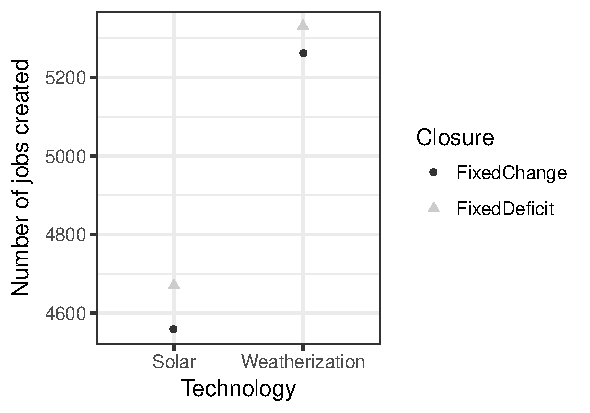
\includegraphics[height=4cm]{figures/closure.pdf}
	\caption{Impact of the trade closure rule}
	\label{fig:closure}
\end{figure}

\subsubsection{Full sensitivity analysis}
\label{sec:full_sensitivity}

\begin{table}
	\small
	\centering
	\caption{Full sensitivity analysis for solar}
	\begin{tabular}{llllllll}
		\toprule
		Techno & gamma & sigma KL & Sigma Armington & Psi CET & CGE Value & IO Value & Ratio \\
		\midrule
		Solar & 0.1 & 0.2 & 1.5 & 1.5 & 6035 & 5010 & 0.83 \\
		Solar & 0.1 & 0.2 & 1.5 & 2 & 5945 & 5010 & 0.84 \\
		Solar & 0.1 & 0.2 & 1.5 & 4 & 5612 & 5010 & 0.89 \\
		Solar & 0.1 & 0.2 & 1.5 & 6 & 5314 & 5010 & 0.94 \\
		Solar & 0.1 & 0.2 & 2 & 1.5 & 5945 & 5010 & 0.84 \\
		Solar & 0.1 & 0.2 & 2 & 2 & 5858 & 5010 & 0.86 \\
		Solar & 0.1 & 0.2 & 2 & 4 & 5534 & 5010 & 0.91 \\
		Solar & 0.1 & 0.2 & 2 & 6 & 5244 & 5010 & 0.96 \\
		Solar & 0.1 & 0.2 & 4 & 1.5 & 5613 & 5010 & 0.89 \\
		Solar & 0.1 & 0.2 & 4 & 2 & 5535 & 5010 & 0.91 \\
		Solar & 0.1 & 0.2 & 4 & 4 & 5245 & 5010 & 0.96 \\
		Solar & 0.1 & 0.2 & 4 & 6 & 4984 & 5010 & 1.01 \\
		Solar & 0.1 & 0.2 & 6 & 1.5 & 5316 & 5010 & 0.94 \\
		Solar & 0.1 & 0.2 & 6 & 2 & 5247 & 5010 & 0.95 \\
		Solar & 0.1 & 0.2 & 6 & 4 & 4985 & 5010 & 1.00 \\
		Solar & 0.1 & 0.2 & 6 & 6 & 4748 & 5010 & 1.06 \\
		Solar & 0.1 & 0.4 & 1.5 & 1.5 & 5130 & 5010 & 0.98 \\
		Solar & 0.1 & 0.4 & 1.5 & 2 & 5066 & 5010 & 0.99 \\
		Solar & 0.1 & 0.4 & 1.5 & 4 & 4823 & 5010 & 1.04 \\
		Solar & 0.1 & 0.4 & 1.5 & 6 & 4603 & 5010 & 1.09 \\
		Solar & 0.1 & 0.4 & 2 & 1.5 & 5066 & 5010 & 0.99 \\
		Solar & 0.1 & 0.4 & 2 & 2 & 5003 & 5010 & 1.00 \\
		Solar & 0.1 & 0.4 & 2 & 4 & 4766 & 5010 & 1.05 \\
		Solar & 0.1 & 0.4 & 2 & 6 & 4551 & 5010 & 1.10 \\
		Solar & 0.1 & 0.4 & 4 & 1.5 & 4824 & 5010 & 1.04 \\
		Solar & 0.1 & 0.4 & 4 & 2 & 4767 & 5010 & 1.05 \\
		Solar & 0.1 & 0.4 & 4 & 4 & 4552 & 5010 & 1.10 \\
		Solar & 0.1 & 0.4 & 4 & 6 & 4355 & 5010 & 1.15 \\
		Solar & 0.1 & 0.4 & 6 & 1.5 & 4605 & 5010 & 1.09 \\
		Solar & 0.1 & 0.4 & 6 & 2 & 4553 & 5010 & 1.10 \\
		Solar & 0.1 & 0.4 & 6 & 4 & 4356 & 5010 & 1.15 \\
		Solar & 0.1 & 0.4 & 6 & 6 & 4175 & 5010 & 1.20 \\
		Solar & 0.1 & 0.6 & 1.5 & 1.5 & 4480 & 5010 & 1.12 \\
		Solar & 0.1 & 0.6 & 1.5 & 2 & 4430 & 5010 & 1.13 \\
		Solar & 0.1 & 0.6 & 1.5 & 4 & 4244 & 5010 & 1.18 \\
		Solar & 0.1 & 0.6 & 1.5 & 6 & 4073 & 5010 & 1.23 \\
		Solar & 0.1 & 0.6 & 2 & 1.5 & 4431 & 5010 & 1.13 \\
		Solar & 0.1 & 0.6 & 2 & 2 & 4382 & 5010 & 1.14 \\
		Solar & 0.1 & 0.6 & 2 & 4 & 4200 & 5010 & 1.19 \\
		Solar & 0.1 & 0.6 & 2 & 6 & 4033 & 5010 & 1.24 \\
		Solar & 0.1 & 0.6 & 4 & 1.5 & 4245 & 5010 & 1.18 \\
		Solar & 0.1 & 0.6 & 4 & 2 & 4201 & 5010 & 1.19 \\
		Solar & 0.1 & 0.6 & 4 & 4 & 4034 & 5010 & 1.24 \\
		Solar & 0.1 & 0.6 & 4 & 6 & 3879 & 5010 & 1.29 \\
		Solar & 0.1 & 0.6 & 6 & 1.5 & 4075 & 5010 & 1.23 \\
		Solar & 0.1 & 0.6 & 6 & 2 & 4035 & 5010 & 1.24 \\
		Solar & 0.1 & 0.6 & 6 & 4 & 3880 & 5010 & 1.29 \\
		Solar & 0.1 & 0.6 & 6 & 6 & 3737 & 5010 & 1.34 \\
		\bottomrule
		\end{tabular}
\end{table}	

\begin{table}
	\small
		\centering
		\caption{Full sensitivity analysis for weatherization}
		\
		\begin{tabular}{llllllll}
		\toprule
		Techno & gamma & sigma KL & Sigma Armington & Psi CET & CGE Value & IO Value & Ratio \\
		\midrule
		Weatherization & 0.1 & 0.2 & 1.5 & 1.5 & 6782 & 8050 & 1.19 \\
		Weatherization & 0.1 & 0.2 & 1.5 & 2 & 6684 & 8050 & 1.20 \\
		Weatherization & 0.1 & 0.2 & 1.5 & 4 & 6321 & 8050 & 1.27 \\
		Weatherization & 0.1 & 0.2 & 1.5 & 6 & 5997 & 8050 & 1.34 \\
		Weatherization & 0.1 & 0.2 & 2 & 1.5 & 6683 & 8050 & 1.20 \\
		Weatherization & 0.1 & 0.2 & 2 & 2 & 6589 & 8050 & 1.22 \\
		Weatherization & 0.1 & 0.2 & 2 & 4 & 6237 & 8050 & 1.29 \\
		Weatherization & 0.1 & 0.2 & 2 & 6 & 5921 & 8050 & 1.36 \\
		Weatherization & 0.1 & 0.2 & 4 & 1.5 & 6321 & 8050 & 1.27 \\
		Weatherization & 0.1 & 0.2 & 4 & 2 & 6236 & 8050 & 1.29 \\
		Weatherization & 0.1 & 0.2 & 4 & 4 & 5921 & 8050 & 1.36 \\
		Weatherization & 0.1 & 0.2 & 4 & 6 & 5637 & 8050 & 1.43 \\
		Weatherization & 0.1 & 0.2 & 6 & 1.5 & 5998 & 8050 & 1.34 \\
		Weatherization & 0.1 & 0.2 & 6 & 2 & 5922 & 8050 & 1.36 \\
		Weatherization & 0.1 & 0.2 & 6 & 4 & 5638 & 8050 & 1.43 \\
		Weatherization & 0.1 & 0.2 & 6 & 6 & 5380 & 8050 & 1.50 \\
		Weatherization & 0.1 & 0.4 & 1.5 & 1.5 & 5824 & 8050 & 1.38 \\
		Weatherization & 0.1 & 0.4 & 1.5 & 2 & 5753 & 8050 & 1.40 \\
		Weatherization & 0.1 & 0.4 & 1.5 & 4 & 5486 & 8050 & 1.47 \\
		Weatherization & 0.1 & 0.4 & 1.5 & 6 & 5244 & 8050 & 1.54 \\
		Weatherization & 0.1 & 0.4 & 2 & 1.5 & 5753 & 8050 & 1.40 \\
		Weatherization & 0.1 & 0.4 & 2 & 2 & 5683 & 8050 & 1.42 \\
		Weatherization & 0.1 & 0.4 & 2 & 4 & 5423 & 8050 & 1.48 \\
		Weatherization & 0.1 & 0.4 & 2 & 6 & 5187 & 8050 & 1.55 \\
		Weatherization & 0.1 & 0.4 & 4 & 1.5 & 5486 & 8050 & 1.47 \\
		Weatherization & 0.1 & 0.4 & 4 & 2 & 5423 & 8050 & 1.48 \\
		Weatherization & 0.1 & 0.4 & 4 & 4 & 5187 & 8050 & 1.55 \\
		Weatherization & 0.1 & 0.4 & 4 & 6 & 4971 & 8050 & 1.62 \\
		Weatherization & 0.1 & 0.4 & 6 & 1.5 & 5245 & 8050 & 1.53 \\
		Weatherization & 0.1 & 0.4 & 6 & 2 & 5188 & 8050 & 1.55 \\
		Weatherization & 0.1 & 0.4 & 6 & 4 & 4972 & 8050 & 1.62 \\
		Weatherization & 0.1 & 0.4 & 6 & 6 & 4774 & 8050 & 1.69 \\
		Weatherization & 0.1 & 0.6 & 1.5 & 1.5 & 5135 & 8050 & 1.57 \\
		Weatherization & 0.1 & 0.6 & 1.5 & 2 & 5080 & 8050 & 1.58 \\
		Weatherization & 0.1 & 0.6 & 1.5 & 4 & 4873 & 8050 & 1.65 \\
		Weatherization & 0.1 & 0.6 & 1.5 & 6 & 4684 & 8050 & 1.72 \\
		Weatherization & 0.1 & 0.6 & 2 & 1.5 & 5080 & 8050 & 1.58 \\
		Weatherization & 0.1 & 0.6 & 2 & 2 & 5026 & 8050 & 1.60 \\
		Weatherization & 0.1 & 0.6 & 2 & 4 & 4824 & 8050 & 1.67 \\
		Weatherization & 0.1 & 0.6 & 2 & 6 & 4639 & 8050 & 1.74 \\
		Weatherization & 0.1 & 0.6 & 4 & 1.5 & 4873 & 8050 & 1.65 \\
		Weatherization & 0.1 & 0.6 & 4 & 2 & 4824 & 8050 & 1.67 \\
		Weatherization & 0.1 & 0.6 & 4 & 4 & 4639 & 8050 & 1.74 \\
		Weatherization & 0.1 & 0.6 & 4 & 6 & 4468 & 8050 & 1.80 \\
		Weatherization & 0.1 & 0.6 & 6 & 1.5 & 4684 & 8050 & 1.72 \\
		Weatherization & 0.1 & 0.6 & 6 & 2 & 4640 & 8050 & 1.74 \\
		Weatherization & 0.1 & 0.6 & 6 & 4 & 4469 & 8050 & 1.80 \\
		Weatherization & 0.1 & 0.6 & 6 & 6 & 4310 & 8050 & 1.87 \\
		\bottomrule
	\end{tabular}
\end{table}

